\documentclass[notitlepage]{article}
\usepackage[margin = 2.5cm]{geometry}
\usepackage[utf8]{inputenc}
\usepackage{graphicx, dcolumn}

\usepackage{booktabs}
\usepackage{siunitx}
\newcolumntype{d}{S[input-symbols = ()]}

\title{Document 1}
\author{Me}
\date{\today}

\begin{document}

\maketitle

\clearpage
\section{Plots}

In this document I show the main plots first, Figure~\ref{fig1} and Figure~\ref{fig2}:

% ----------------------------------------------------
\begin{figure*}[htb!]
  \centering

  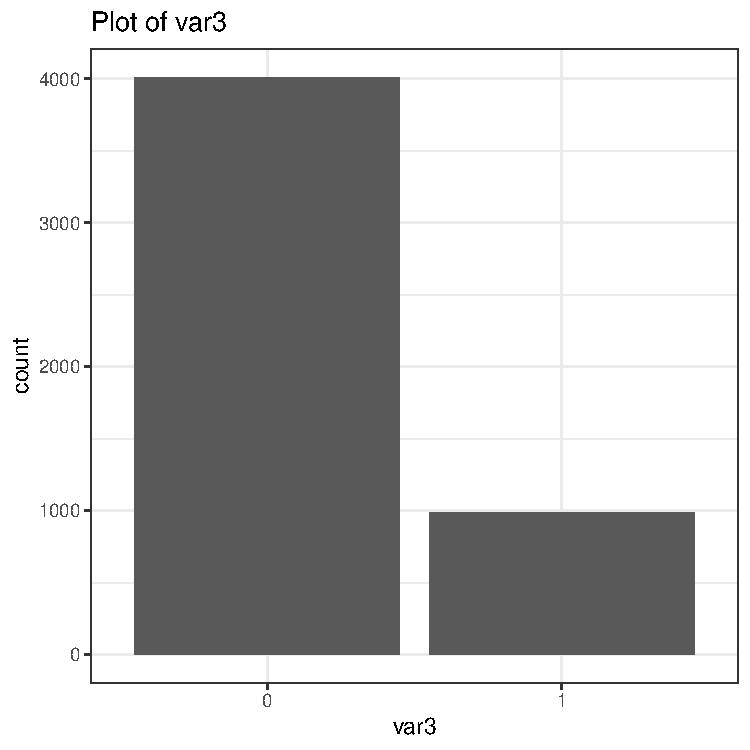
\includegraphics[width = 0.5\textwidth]{../plots/output/histogram}

  \caption{Histogram}\label{fig1}
\end{figure*}
% ----------------------------------------------------

% ----------------------------------------------------
\begin{figure*}[htb!]
  \centering

  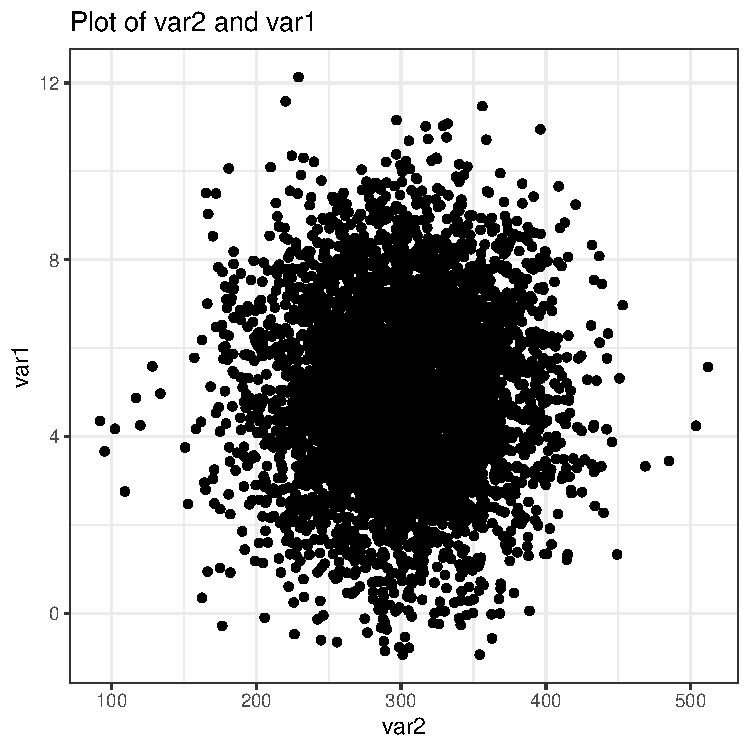
\includegraphics[width = 0.5\textwidth]{../plots/output/scatterplot}

  \caption{Scatter}\label{fig2}
\end{figure*}
% ----------------------------------------------------

\clearpage
\section{Models}

And then I show the table with the models results:

\begin{table}
\centering
\begin{tabular}[t]{lcc}
\toprule
  & Model 1 & Model 2\\
\midrule
Variable 2 & \num{0.001}+ & \num{0.001}+\\
 & (\num{0.001}) & (\num{0.001})\\
Variable 3 &  & \num{-0.182}**\\
 &  & (\num{0.070})\\
\midrule
Num.Obs. & \num{5000} & \num{5000}\\
R2 & \num{0.001} & \num{0.002}\\
R2 Adj. & \num{0.000} & \num{0.002}\\
AIC & \num{21029.0} & \num{21024.2}\\
BIC & \num{21048.5} & \num{21050.3}\\
RMSE & \num{1.98} & \num{1.98}\\
\bottomrule
\end{tabular}
\end{table}


\end{document}
